\section{Localisation en intérieur}
Un challenge principal était la localisation en intérieur de l'utilisateur. C'est intéressant pour l'utilisateur s'il a un suivi régulier de sa position durant la visualisation 3D. Cette section va expliquer les diverses pistes empruntées ainsi que leurs résultats.

\subsection{GPS}
Quand on entend localisation on pense très vite au GPS (\textit{Global Positioning System}) qui pourrait présenter une bonne solution à première vue. Cependant cette technologie manque de précision, principalement en intérieur. La précision des GPS mobiles se situerait à peu près entre 4 et 50 mètres, dépendant des conditions et du smartphone utilisé. En général, l'erreur est due aux éléments entre l'utilisateur et le satellite, c'est pourquoi la localisation en intérieur ne peut pas se fier au GPS.

\subsection{Triangulation Wifi}
Une méthode utilisé pour la localisation en intérieur est la triangulation / trilateration en utilisant les \textit{Access Points} WiFi. Le concept est d'avoir à l'avance retenu les coordonnées de tous les AP. Chaque AP possède une adresse MAC qui les différencie les uns des autres. Ensuite il faut scanner les AP depuis l'objet que l'ont veut localiser et en fonction des forces des AP il est possible de retrouver sa position.

L'avantage de cette solution est qu'il n'y a pas d'infrastructure à mettre en place, étant donné que le Campus est déjà équipé de bon nombre d'AP. Cependant le but de ce projet est d'offrir une application dans un navigateur Internet. Cette contrainte nous empêche d'accéder à n'importe quelle information de l'appareil qui l'utilise. Malgré les technologies qu'offre ce monde il est encore impossible de récupérer les informations nécessaires à la triangulation / trilatération depuis une page web.

\subsection{Triangulation Bluetooth}
Une autre manière d'utiliser la triangulation est de mettre en place des beacons bluetooth. Il s'agit de petits émetteurs que l'on place dans l'espace où l'on veut localiser l'utilisateur. Le fonctionnement de la triangulation est pareil que pour le WiFi.


Sans compter le désavantage qu'est la mise en place de l'infrastructure, les accès bluetooth depuis une page web ne sont pas encore assez supportés. Le tableau \ref{caniuse-bluetooth} tiré du site www.caniuse.com montre que seul Chrome le supporte ssi on active le drapeau nécessaire. Ceci démontre que l'API Web Bluetooth n'est pas utilisable pour une application destinée au grand public.

\begin{figure}[h!]
	\center
	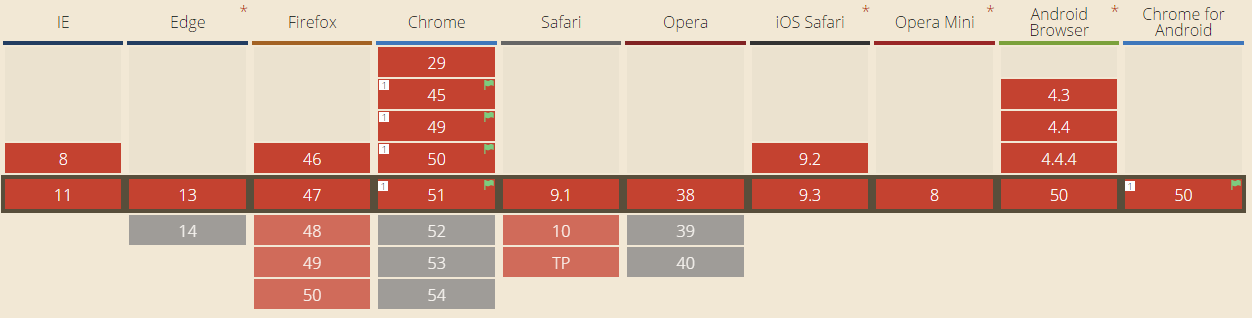
\includegraphics[width=10cm,frame]{caniuse_bluetooth}
	\caption{Support de l'API Web Bluetooth par les différents navigateurs.}
	\label{caniuse-bluetooth}
\end{figure}

\subsection{Accéléromètre et Gyroscope}
L'approche ici est différente, nous désirons utiliser les capteurs internes du smartphone afin de calculer une position. HTML5 fournit une API pour détecter l'orientation et les déplacements du dispositif. Autrement dit, nous avons accès à l'accéléromètre et au gyroscope depuis un navigateur Internet.

A l'aide de l'accélération il est théoriquement possible de calculer une position. Cependant les valeurs de ces capteurs comportent un bruit et pour calculer une position il faut double-intégrer l'accélération. Cela signifie que nous devrons double-intégrer le bruit et cela va créer un \textit{drift}, en quelques secondes l'erreur peut s'élever à une vingtaine de centimètres. En outre, le gyroscope peut avoir une valeur erronée due à la suppression de la gravité. C'est-à-dire que si nous avons une erreur d'un degré sur la valeur du gyroscope, en quelques seconde l'erreur s'élève à plusieurs mètres cette fois. Citer https://youtu.be/C7JQ7Rpwn2k?t=23m22s

Le but de cette approche était d'estimer la position de l'utilisateur sans pour autant connaître la valeur exacte. Les résultats prouvent que même une approximation n'est pas envisageable avec ces capteurs.